\documentclass[12pt]{article}

\usepackage[margin=1in]{geometry}  % set the margins to 1in on all sides
\usepackage{graphicx}              % to include figures
\usepackage{amsmath}               % great math stuff
\usepackage{amsfonts}              % for blackboard bold, etc
\usepackage{amsthm}                % better theorem environments
\usepackage{bm}					   % bm for bold math

\usepackage{enumitem} % for [noitemsep]
\usepackage{rotating} % for sideway table
\usepackage{caption} % for newline in caption
\usepackage{xcolor}
\usepackage{hyperref}
\hypersetup{
    colorlinks,
    linkcolor={red!50!black},
    citecolor={blue!50!black},
    urlcolor={blue!80!black}
}
\usepackage{cleveref}

\usepackage{placeins}  
\usepackage{float}
\restylefloat{table}

% bibliography
\usepackage{natbib}
\bibpunct{(}{)}{;}{a}{}{,} % no comma between author and year

\title{Two-Sided Matching Model}
\author{Anh Le}

\begin{document}
\maketitle

Since the last few days I have the following findings / improvements:

\section{MCMC chains for employers' preference $\alpha$}

I had a hunch that the conditional logit side of the model does not work well
when the choices' covariates only vary across choices and NOT across choosers.
In the labor market example, it means that a job's characteristics appear the
same to different workers. In the FDI market example, it means that a country's
characteristics appear the same to different multinationals.

While many texts on conditional logit model say that this is fine, my simulation
of one-sided conditional logit shows that the MLE is very imprecise, albeit
unbiased. This could cause the MCMC to venture into very far-off region.

So I simulate my own two-sided market, with agents on two sides making,
evaluating, and accepting offers, where the choices' covariates vary across
choosers as well. In the job market example, it means that company offers
slightly different jobs to different employees.

As shown below, the MCMC chains are remarkably better. They actually converge to
the true parameter values now instead of behaving very poorly as before. This is
evidence that my math and my implementation are correct.

But I'm still theoretically confused about the need for the choices' covariates
to vary across choosers. If that's a requirement, the data requirement of the
model is now tougher, as we need the characteristics of the jobs
(or countries) to vary across workers (or multinationals) somehow.

\begin{figure}[!ht]
\centering
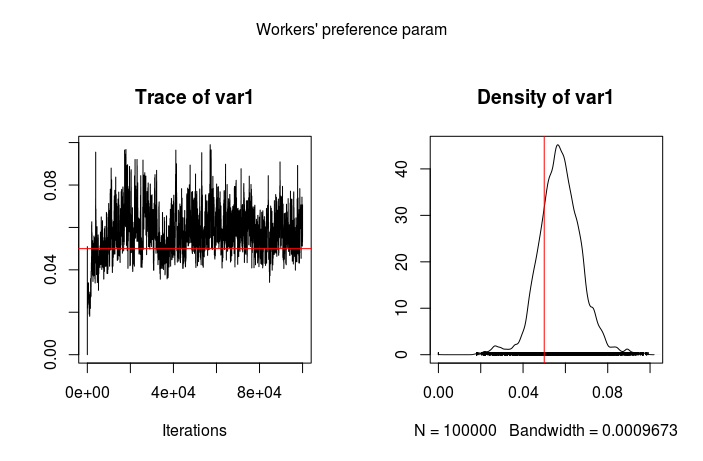
\includegraphics[width=0.8\textwidth]{../figure/worker_alpha_starting_opp}
\caption{Using hand-crafted opportunity set}
\end{figure}

\begin{figure}[!ht]
\centering
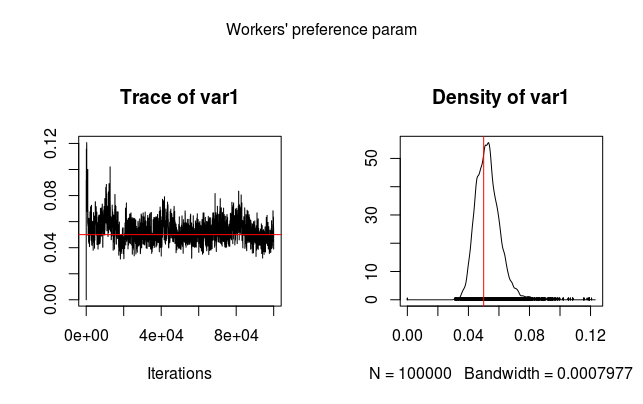
\includegraphics[width=0.8\textwidth]{../figure/worker_alpha_obs_opp}
\caption{Using the observed opportunity set}
\end{figure}

\FloatBarrier
\section{MCMC chains for employers' preference $\beta$}

Since I'm simulating the data, I was able to choose sensible scale for the
proposal distribution, helping $\beta$ slowly converge towards their true
values. When the proposal values of $\beta$ manage to get accepted, the proposal
values of the opportunity set also do.

But I'm concerned about choosing the right scale for the $\beta$ in the real
dataset. Since the parameters in the random utility models like these only have
meaning relative to one another, it seems difficult to reason through what their magnitude
may be. This problem exacerbates when real data has 20 employers (or 30
countries), rather than 5 simulated employers here. In theory, an adaptive procedure would help, but past
experience suggests that it could only help if the initial, non-adapted part of
the MCMC went well.

\begin{figure}[!ht]
\centering
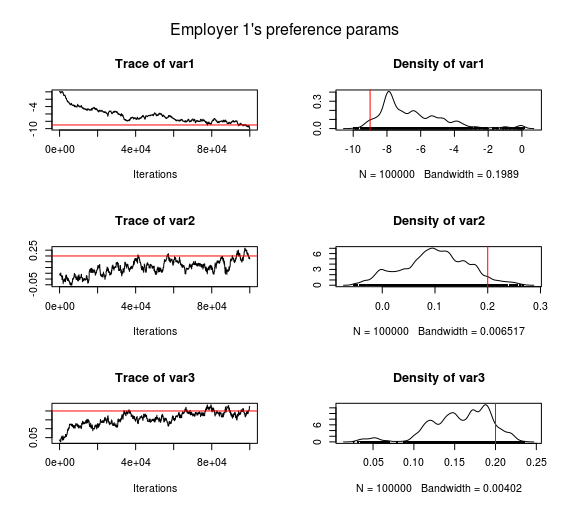
\includegraphics[width=0.8\textwidth]{../figure/employer1_beta_starting_opp}
\caption{Using hand-crafted opportunity set}
\end{figure}

\begin{figure}[!ht]
\centering
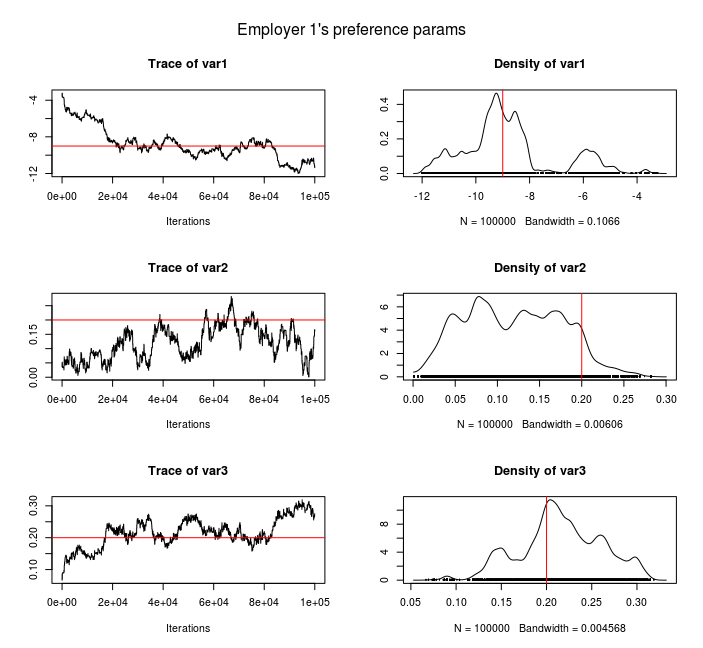
\includegraphics[width=0.8\textwidth]{../figure/employer1_beta_obs_opp}
\caption{Using the observed opportunity set}
\end{figure}

\FloatBarrier
\section{Monitoring the convergence of the opportunity set}

It's also difficult to check if the MCMC for the opportunity set is doing well.
The opportunity set is a binary matrix, and below I check various statistics
regarding how different the current set is from the true, simulated set. (It's
actually quite different -- which is confusing given that $\beta$ seems to get
closer to the true value later in the chain).
However, for real data, I'm not sure how to monitor the convergence of the
opportunity set.

\begin{figure}[!ht]
\centering
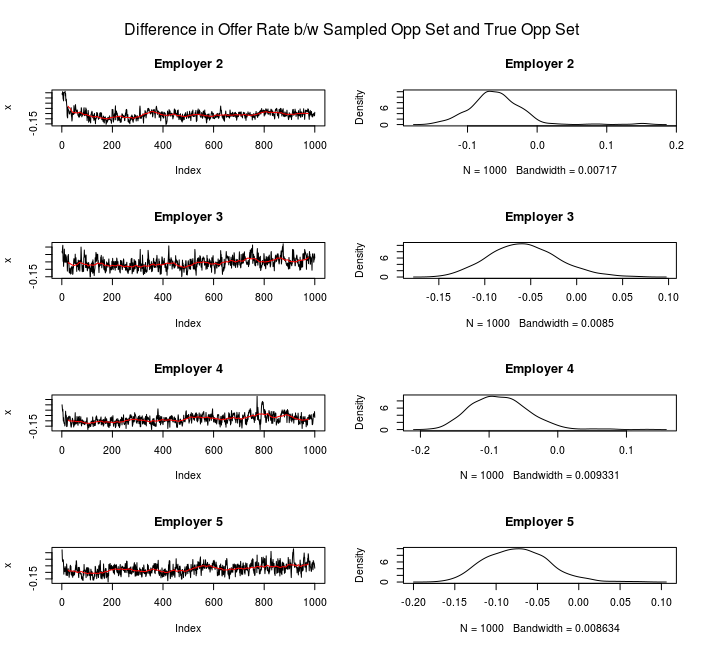
\includegraphics[width=0.8\textwidth]{../figure/diff_offer_rate_opp_starting_opp}
\caption{Using hand-crafted opportunity set}
\end{figure}

\begin{figure}[!ht]
\centering
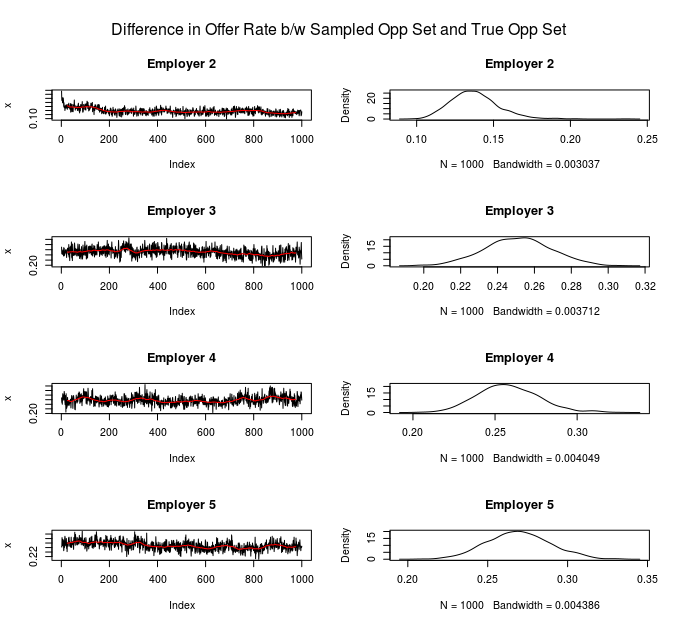
\includegraphics[width=0.8\textwidth]{../figure/diff_offer_rate_opp_obs_opp}
\caption{Using the observed opportunity set}
\end{figure}

\begin{figure}[!ht]
\centering
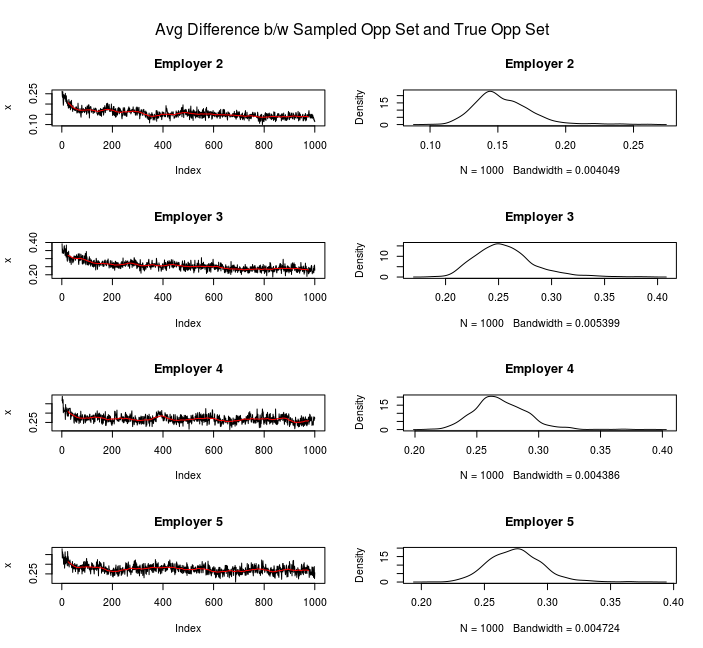
\includegraphics[width=0.8\textwidth]{../figure/avg_diff_opp_starting_opp}
\caption{Using hand-crafted opportunity set}
\end{figure}

\begin{figure}[!ht]
\centering
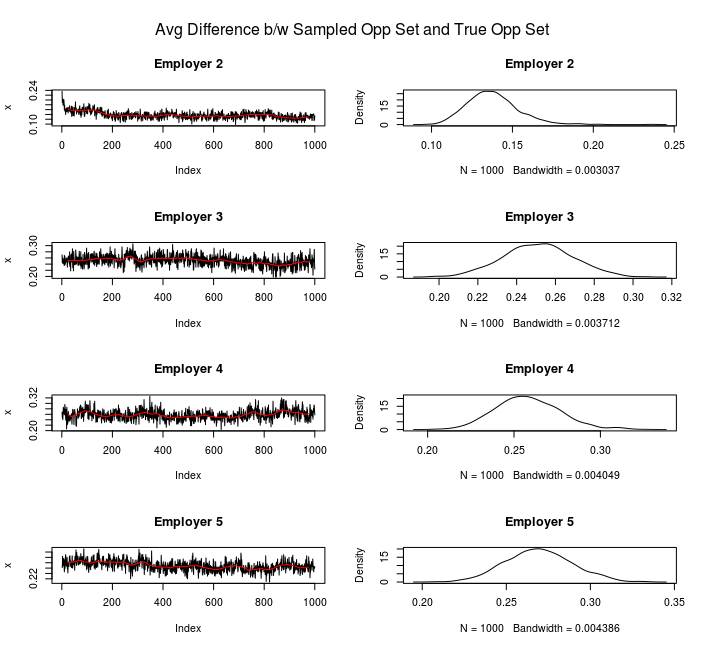
\includegraphics[width=0.8\textwidth]{../figure/avg_diff_opp_obs_opp}
\caption{Using the observed opportunity set}
\end{figure}

\clearpage
\bibliographystyle{chicago}
\bibliography{library}
\end{document}